\chapter{Teorema de Lax-Milgran}

Para dejar el puente libre, primero necesitamos ver nuestro funcional $L$ desde otro punto de vista. Para ello, vamos a ver una serie de definiciones y propiedades abstractas sobre los \textit{funcionales cuadráticos}, lo que nos va a permitir enunciar el teorema de Lax-Milgran, que nos dará la existencia de solución en esta última versión del modelo.

\begin{definition}\label{formabilineal}
Dados un cuerpo $K$ y un $K-$espacio vectorial $V$, una forma bilineal es una aplicación $\funcion{f}{V\times V}{K}$ que verifica:
\begin{enumerate}[(a)]
\item $f(u_1+u_2,v)=f(u_1,v)+f(u_2,v)$
\item $f(u, v_1+v_2)=f(u,v_1)+f(u,v_2)$
\item $f(au,v)=af(u,v)$
\item $f(u,av)=af(u,v)$
\end{enumerate}
para cualquier $a\in K$ y $u,v,u_1,u_2,v_1,v_2\in V$.

Una propiedad que necesitaremos es:
\[
f\left(\sum_ia_iu_i,\sum_jb_jv_h\right)=\sum_i\sum_ja_ib_jf(u_i,v_j)
\]

\end{definition}

\begin{definition}
Una forma bilineal $\funcion{f}{V\times V}{K}$ se dice simétrice si verifica:
\[
f(u,v)=f(v,u) \espacio \forall u,v\in V
\]
\end{definition}

\begin{definition}
Sea $H$ un espacio de Hilbert arbitrario, $\funcion{A}{H\times H}{\R}$ una forma bilineal, continua y simétrica y $\funcion{R}{H}{\R}$ una aplicación lineal y continua. Llamamos funcional cuadrático a la aplicación $\funcion{L}{H}{\R}$ dada por
\[
L(y)=\frac{1}{2}A(y,y)-R(y) \espacio\forall y\in H
\]
\end{definition}

\begin{definition}
Sea $\funcion{L}{H}{\R}$ una forma cuadrática. Diremos que es coerciva si existe una constante $\alpha\in\R^+$ tal que:
\[
A(u,u)\geq \alpha\norm{u}^2 \espacio \forall u\in H
\]
\end{definition}

\begin{prop}
Sea un espacio de Hilbert $H$ y $\funcion{L}{H}{\R}$ una forma cuadrátrica en ese espacio.
Entonces, la aplicación $\funcion{\norm{\cdot}_H}{H}{\R^+_0}$ definida por 
\[
\norm{u}_H=\sqrt{A(u,u)} \espacio \forall u\in H
\]
donde $\funcion{A}{H\times H}{\R}$ es la forma bilineal asociada a $L$, es una norma, y es equivalente a la norma natural de $H$.
\end{prop}
\begin{proof}
El hecho de que $\norm{\cdot}_H$ es una norma es sencillo de comprobar ya que $A$ define un producto escalar en $H$.

Sea $\funcion{\norm{\cdot}}{H}{\R}$ la norma de $H$. Necesitamos encontrar dos constante $c_1,c_2\in\R^+$ tal que 
\[
c_1\norm{u}\leq \norm{u}_H \leq c_2\norm{u}
\]
La constante $c_2$ la obtenemos por continuidad de la norma $\norm{\cdot}_H$ y la constante $c_1$ de la coercividad de $L$.

\end{proof}
A partir de ahora consideramos $\norm{\cdot}_H$ como nuestra norma por defecto en $H$.
\begin{prop}
Todo funcional cuadrático coercivo está acotado inferiormente.
\end{prop}
\begin{proof}
Sea $\funcion{L}{H}{\R}$ un funcional cuadrático, donde $\funcion{A}{H\times H}{\R}$ es su forma bilineal, continua y simétrica y $\funcion{R}{H}{\R}$ es su aplicación lineal y continua.
Vamos a ver que podemos acotar inferiormente la expresión de $L(y)$, con $y\in H$, por una función parabólica hacia arriba.

Como $R$ es continua, entonces $\norm{R(y)}\leq \norm{R}\norm{y} \Rightarrow -\norm{R(y)} \geq -\norm{R}\norm{y}$. Además, como $L$ es coerciva, existe cierta constante $C\in\R^+$ tal que $A(y,y)\geq C\norm{y}^2$. Combinando esas dos acotaciones, obtenemos:
\[
L(y)=\frac{1}{2}A(y,y)-R(y)\geq \frac{1}{2}C\norm{y}^2-\norm{R}\norm{y}
\]
Para ver con más claridad la parábola, hacemos el cambio $s=\norm{y}$, obteniendo una nueva función $P$ dependiente de las dos constantes $C$ y $\norm{R}$: $P(s)=\frac{1}{2}s^2-s\norm{R}$. Derivando e igualando a 0, obtenemos fácilmente que el mínimo de la parábola $P$ se alcanza en $s=\frac{\norm{R}}{C}$. Luego:
\[
L(y)\geq \frac{\norm{R}}{C} \espacio \forall y\in H 
\]

\end{proof}

\begin{theorem}[Lax-Milgran]
\label{laxmilgran}
Sea $\funcion{L}{H}{\R}$ un funcional cuadrático. Si $L$ es coercivo, entonces tiene mínimo absoluto en $H$.
\end{theorem}

\begin{prop}[condición de punto crítico]
\label{puntocritico}
Sea $\funcion{L}{H}{\R}$ un funcional cuadrático coercivo, $y\in H$, $\phi\in\soportecompacto$. Entonces existe $y\in H$ verificando:
\[
A(\phi,y)-R(\phi)=0 \espacio \forall\phi\in\soportecompacto
\]

Además, el punto $y$ es el mínimo de $L$.
\end{prop}
\begin{proof}
Calculemos primero la expresión explícita de $g(s)$:
\[
g(s)=L(y+s\phi)=\frac{1}{2}A(y+s\phi,y+s\phi)-R(y+s\phi)
\]
Desarrollamos el primer término (usando la última propiedad en la definición \ref{formabilineal}):
\[
A(y+s\phi,y+s\phi)=A(y,y)+sA(y,\phi)+sA(\phi,y)+s^2A(\phi,\phi)=s^2A(\phi,\phi)+2sA(\phi,\phi)+A(y,y)
\]
Para el segundo término, usamos que $R$ es lineal:
\[
R(y+s\phi)=R(y)+sR(\phi)
\]
Quedándo:
\[
g(s)=\frac{1}{2}\left(s^2A(\phi,y)+2sA(\phi,\phi)+A(y,y)\right)-R(y)-sR(\phi)
\]
Derivando respecto de $s$:
\[
g(s)=sA(\phi,\phi)+A(\phi,y)-R(\phi) \Rightarrow g'(0)=A(\phi,y)-R(\phi)
\]
Luego nuestra condición de punto crítico es:
\[
A(\phi,y)-R(\phi)=0 \espacio \forall\phi\in\soportecompacto
\]

Para le existencia, simplemente tenemos que definir un producto escalar y usar el teorema de Riesz, como en los ejemplos anteriores. Sea $<<u,v>>=A(u,v)$ un producto escalar en $H$, por el teorema \ref{riesz-frechet}, existe $y\in H$ verificando:
\[
<<y,\phi>>=R(\phi) \espacio \forall \phi\in\soportecompacto
\]

Para ver que es mínimo, tomamos $\funcion{g}{\R}{\R}$ definida por $g(s)=L(y+s(z-y))$. Notemos que $y+s(z-y)$ es la recta que una a $z$ con $y$. Tenemos que ver
\[
L(z)>L(y) \espacio \forall z\in H
\]
Que si nos fijamos, es equivalente a ver que
\[
g(1)>g(0)
\]
Que ya lo tenemos porque $s=0$ era el punto mínimo de la parábola.
\end{proof}

Una vez planteada toda la teoría necesaria, podemos volver a nuestro modelo del puente. Recordemos que nuestro funcional  $\funcion{L}{\sobolev{1}}{\R}$ venía dado por la expresión:
\[
L(y)=\frac{1}{2}\integral{a}{b}{y'(x)^2dx}+\frac{1}{2}\integral{a}{b}{K(x)y(x)^2dx}+\integral{a}{b}{q(x)y(x)dx}
\]
donde $q,K\in\lebesgue{\infty}$ y $K(x)\geq k_0 >0\ \casipordoquier$. La última condición la imponemos porque al dejar los extremos sueltos (lo hemos hecho al considerar como dominio de $L$ el espacio $\sobolev{1}$ en lugar de $\sobolevcero{1}$) necesitemos que el puente siga enganchado por las cuerdas.

Para poder usar la teoría desarrollada anteriormente, necesitamos ver que nuestro funcional es cuadrático. Definimos nuestra forma bilineal, continua y simétrica, y nuestra aplicación lineal y continua:
\[
A(u,v)=\integral{a}{b}{u'(x)v'(x)dx}+\integral{a}{b}{K(x)u(x)v(x)dx}, \; \espacio R(u)=-\integral{a}{b}{q(x)u(x)dx} \;\;\forall u,v\in\sobolev{1}
\]
Pero también necesitamos que $L$ sea coerciva. Usando la hipótesis sobre $K(x)$ es fácil de ver:
\[
A(u,u)=\integral{a}{b}{u'(x)^2dx}+\integral{a}{b}{K(x)u(x)^2dx}\geq\normasobolev{1}{u}^2+k_0\normasobolev{1}{u}^2\geq(1+k_0)\normasobolev{1}{u}^2
\]
Por lo tanto, sabemos que existe mínimo en $\sobolev{1}$. Además de saber que existe, queremos saber algo más sobre su expresión. Como hemos visto antes, los puntos críticos están caracterizados por la expresión:
\[
y\in\sobolev{1} \text{ punto critico } \Leftrightarrow A(y,\phi)=R(\phi) \espacio \forall \phi\in\sobolev{1}
\]
es decir,
\[
\integral{a}{b}{y'(x)\phi'(x)dx}+\integral{a}{b}{K(x)y(x)\phi(x)dx}=-\integral{a}{b}{q(x)\phi(x)dx} \espacio  \forall\phi\in\sobolev{1}
\]
Si en lugar de considerar $\phi$ en $\sobolev{1}$, la consideramos en $\soportecompacto$. Vemos que llamando $z=y'$ y agrupando los términos que tienen $\phi$, llegamos a:
\[
\integral{a}{b}{z(x)\phi'(x)dx}=-\integral{a}{b}{(K(x)y(x)+q(x))\phi(x)dx} \espacio  \forall\phi\in\sobolev{1}
\]

lo que significa que la derivada débil de $z$ es justamente $ky+q$. En particular z está en $\sobolev{1}$, porque todas las funciones que aparecen están en $\lebesgue{2}$. Luego debemos resolver la siguiente ecuación diferencial de orden 2 en $y$:
\[
y''(x)=K(x)y(x)+q(x) \espacio \forall x \in[a,b]
\]
Si imaginamos que $K$ y $q$ son continuas, esa ecuación tendría un gran número de soluciones. De hecho, el conjunto de soluciones sería un espacio biparamétrico (porque la solución depende de las condiciones iniciales sobre $y$ e $y'$). Tenemos que intentar limitarlas de alguna forma.

\begin{prop}\label{productoh1}
Sea $y\in\sobolev{1}$ (el representante continuo) y $\phi\in\mathcal{D}(\R)$, entonces $y\phi\in\sobolev{1}$.
\end{prop}
\begin{proof}
Para ver que $y\phi\in\sobolev{1}$, necesitamos encontrar su derivada débil. ¿Cuál es nuestro candidato a derivada débil? La derivada clásica, es decir, $z=y'\phi+y\phi'$. Para comprobarlo, tenemos que ver que para toda $\psi\in\soportecompacto$ se tiene:

\[
\integral{a}{b}{(y'(x)\phi(x)+y(x)\phi'(x))\psi(x)dx}+\integral{a}{b}{y(x)\phi(x)\psi'(x)dx}=0
\]
Reordenando los términos que tienen $y$ e $y'$, obtenemos:
\[
\integral{a}{b}{[\phi(x)\psi'(x)+\phi'(x)\psi(x)]y(x)dx}+\integral{a}{b}{[\phi(x)\psi(x)]y'(x)dx}=0
\]
Se cumple que si
$\phi \in \mathcal{D}(\mathbb{R}), \psi \in \mathcal{D}((a,b))$
entonce $\phi\psi \in \mathcal{D}((a,b))$ y
\[
  (\phi\psi)' = \phi'\psi + \phi\psi'
\]
Ahora por ser $y \in \mathcal{H}^1(a,b)$ y
$\hat\phi \in \mathcal{\mathbb{R}}$ tenemos que se cumple
\[
\integral{a}{b}{y'(x)\hat\phi(x)}+\integral{a}{b}{y(x)\hat\phi'(x)}=y(x)\hat\phi(x)\Big|^b_a
\]
una expresión general. Tomando $\hat\phi = \phi\psi$ tenemos que 

\[
\integral{a}{b}{y'(x)\hat\phi(x)}+\integral{a}{b}{y(x)\hat\phi'(x)}=y(x)\hat\phi(x)\Big|^b_a = 0
\]
ya que $\phi\psi(b) = \phi\psi(a) = 0$ y obtenemos así el resultado que buscabamos.
\end{proof}

Volviendo al problema original teníamos que

\begin{equation}
  \label{eq:probleminicial}
  \integral{a}{b}{y'(x)\phi(x)}+\integral{a}{b}{k(x)y(x)\phi(x)}=-\integral{a}{b}{q(x)\phi(x)}
\end{equation}


Considerando $\phi \in \mathcal{D}(\mathbb{R}), \phi \in \mathcal{H}^1$ y $z = y'$

obtenemos en la expresión anterior

\begin{equation}
  \label{eq:resparcial}
  \integral{a}{b}{z\phi'}=z\phi(x)\Big|^b_a - \integral{a}{b}{z'\phi}
\end{equation}

Como estabamos resolviendo el problema $y''=ky + q$ tenemos que se cumple

\[
\integral{a}{b}{z'\phi} = \integral{a}{b}{k(x)y(x)+q(x)\phi}
\]

y usando la igualdad que nos da \ref{eq:probleminicial} despejamos en
\ref{eq:resparcial} y obtenemos
\[
y'\phi\Big|^b_a = 0
\]

Si tomamos una $\phi$ como la siguiente

\centerline{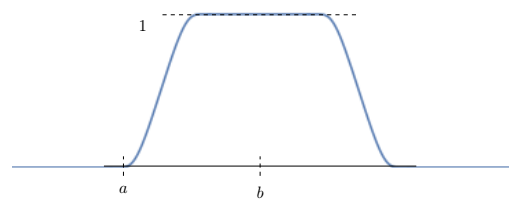
\includegraphics[scale=0.5]{img/caso1.png}} 

de la expresión $ 0 = y'\phi\Big|^b_a = y'(b)\phi(b)-y'(a)\phi(a)$
obtenemos $y'(b) = 0$. Tomando como $\phi$

\centerline{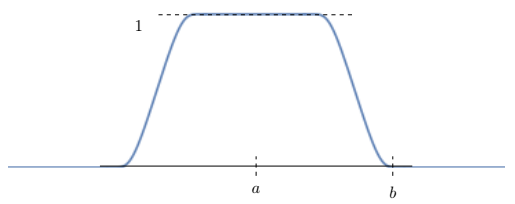
\includegraphics[scale=0.5]{img/caso2.png}} 

obtenemos $y'(a) = 0$. Dado que $z=y'\in \mathcal{H}^1$ entonces $y\in \mathcal{H}^2$ y
tomando el representante continuo obtenemos lo que se conoce como la condición de Neumann.

\section{La delta de Dirac y el espacio $H^{-1}$}

Ahora vamos a ver otro caso del modelo, donde colgamos una masa $m$ en un punto $\alpha\in(a,b)$ del puente. La energía de este objeto es $my(\alpha)$, luego la expresión de nuestro funcional $\funcion{L}{\sobolevcero{1}}{\R}$ es:
\[
L(y)=\frac{1}{2}\integral{a}{b}{y'(x)^2dx}+\frac{1}{2}\integral{a}{b}{q(x)y(x)^2dx}+my(\alpha)
\]
donde $y\in\sobolevcero{1}$, $q(x)\geq 0$ y  $q\in\lebesgue{\infty}$. La intuición nos dice que al colgar la masa $m$, se formará un pico en la cuerda, como muestra el siguiente dibujo:

\begin{center}
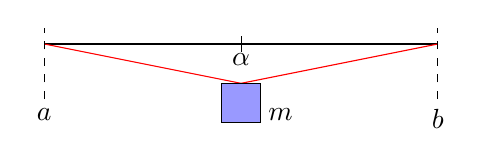
\begin{tikzpicture}
\draw (0,0) -- (5,0);
% parabola
\draw[scale=1,domain=0:2.5,smooth,variable=\x,red] plot ({\x}, {-0.2*\x});
\draw[scale=1,domain=2.5:5,smooth,variable=\x,red] plot ({\x}, {0.2*(\x-5)});

% etiquetas
\draw[dashed] (0,-0.7) -- (0,.2);
\draw (0,-0.7) node[anchor=north] {$a$};
\draw[dashed] (5,-.7) -- (5,.2);
\draw (5,-0.7) node[anchor=north] {$b$};
\draw (2.5,-0.1) -- (2.5,.1);
\draw (2.5,0) node[anchor=north] {$\alpha$};
\draw (3,-0.7) node[anchor=north] {$m$};

% masa
\fill[blue!40!white, draw=black] (2.25,-1) rectangle (2.75,-0.5);
\end{tikzpicture}
\end{center}
La forma bilineal $A$ es la misma que en el anterior modelo:
\[
A(y,y)=\frac{1}{2}\integral{a}{b}{y'(x)^2dx}+\frac{1}{2}\integral{a}{b}{q(x)y(x)^2dx}
\]
y como estamos en $\sobolevcero{1}$, $\integral{a}{b}{y'(x)^2dx}$ es una norma, luego $A$ es coercivo ya que restando el último término (que es positivo) obtenemos:
\[
A(y,y)\geq \frac{1}{2}\integral{a}{b}{y'(x)^2dx} = \frac{1}{2}\norm{u}^2
\] 
La aplicación lineal y continua $\funcion{R}{\sobolevcero{1}}{\R}$, viene dada por $R(y)=-my(\alpha)$, que tiene sentido al elegir el represante continuo porque $\sobolev{1}\subset \mathcal{C}(a,b)$. Por el teorema de Lax-Milgran (\ref{laxmilgran}) y la proposicion \ref{puntocritico}, existe $y\in\sobolevcero{1}$ de forma que
\[
A(y,\phi)=R(\phi) \espacio \forall \phi\in\sobolevcero{1}
\]
Lo que vamos a hacer ahora es calcular o ver qué condiciones verifica la función $y$. Usando la condición de punto crítico:
\begin{equation}
\label{formulageneral}
\integral{a}{b}{y'(x)\phi'(x)dx}+\integral{a}{b}{q(x)y(x)\phi(x)dx}=-m\phi(\alpha)
\end{equation}
Ahora hacemos una distinción de casos con $\phi$ perteneciendo a diferentes clases de Swartz:
\begin{itemize}[-]
\item si $\phi\in\mathcal{D}(a,\alpha)$:
\[
\integral{a}{b}{y'(x)\phi'(x)dx}+\integral{a}{b}{q(x)y(x)\phi(x)dx}=-m\phi(\alpha)=0
\]
ya que $\alpha\notin(a,\alpha) \Rightarrow \phi(\alpha)=0$. Si denotamos $z=y'$, entonces $z\in\sobolev[a,\alpha]{1}\subset\mathcal{C}[a,\alpha]$ (porque la expresión anterior coincide con la definición de derivada débil para $z$).
\item si $\phi\in\mathcal{D}(\alpha,b)$, de igual forma conseguimos que $z\in\sobolevcero[\alpha,b]{1}\subset\mathcal{C}[\alpha,b]$. 
\end{itemize}
Fijaros que ese razonamiento no implica que $z\in\mathcal{C}[a,b]$, ya que el representante continuo usado en $[a,\alpha]$ y $[\alpha,b]$ son distintos. Lo que si implica es que $z\in\mathcal{C}\left([a,\alpha]\right)\cap \mathcal{C}\left([\alpha,b]\right)$ y existen los límites laterales de $\alpha$:
\[
z(\alpha^-)=\limite{x}{\alpha^-}{z(x)} \espacio z(\alpha^+)=\limite{x}{\alpha^+}{z(x)}
\]
Además sabemos que $z'=qy \;\; a.e \; x \in(a,\alpha)\cup(\alpha,b)$. Si volvemos a la fórmula general \eqref{formulageneral}:
\begin{equation}
\label{formulageneral2}
\integral{a}{b}{z(x)\phi'(x)dx}+\integral{a}{b}{q(x)y(x)\phi(x)dx}=-m\phi(\alpha) \espacio \forall\phi\in\sobolevcero{1}
\end{equation}
Ahora queremos desarrollar esa expresión. Tomamos $\phi\in\soportecompacto$, como $z$ no es continua en $\alpha$, la integral del primer término hay que escribirla en dos partes:
\[
\integral{a}{b}{z(x)\phi'(x)dx}=\integral{a}{\alpha}{z(x)\phi'(x)dx}+\integral{\alpha}{b}{z(x)\phi'(x)dx}
\]
Aplicamos derivación por partes a cada término:
\[
\integral{a}{\alpha}{z(x)\phi'(x)dx}=z(x)\phi(x)\Big|_a^\alpha-\integral{a}{\alpha}{z'(x)\phi(x)dx}=z(\alpha^-)\phi(\alpha)-\integral{a}{\alpha}{z'(x)\phi(x)dx}
\]
\[
\integral{\alpha}{b}{z(x)\phi'(x)dx}=z(x)\phi(x)\Big|_\alpha^b-\integral{\alpha}{b}{z'(x)\phi(x)dx}=-z(\alpha^+)\phi(\alpha)-\integral{\alpha}{b}{z'(x)\phi(x)dx}
\]
Combinando los resultados y sustituyendo en \eqref{formulageneral2}:
\[
z(\alpha^-)\phi(\alpha)-z(\alpha^+)\phi(\alpha)-\integral{a}{b}{z'(x)\phi(x)dx}=-\integral{a}{b}{z'(x)\phi(x)dx}-m\phi(\alpha)
\]
Cancelando ámbos términos:
\[
\left(z(\alpha^-)-z(\alpha^+)\right)\phi(\alpha)=-m\phi(\alpha)
\]
Como la función de Swartz escogida es arbitraria, podemos suponer que vale 1 en $\alpha$. Usando eso y que $z=y'$:
\[
y'(\alpha^-)-y'(\alpha^+)=-m \Rightarrow y'(\alpha^+)-y'(\alpha^-)=m  
\]
Es decir, el cambio de pendiente que se da entre $\alpha^-$ y $\alpha^+$ es igual a $m$, el peso de la masa.

\section{Sturm-Liouville: caso 1}

Vamos a generalizar el caso anterior para obtener una ecuación diferencial con varias condiciones. Sea $\funcion{L}{\sobolev{1}}{\R}$ el funcional dado por:
\[
L(y)=\frac{1}{2}\integral{a}{b}{y'(x)^2dx}+\frac{1}{2}\integral{a}{b}{q(x)y(x)^2dx}-R(y)
\]
con $q\in\lebesgue{\infty}$, $0<q_0\leq q(x)\leq q_1 \; \casipordoquier$. 

De donde podemos definir la siguiente forma cuadrática: 
\[
A(y,\phi)=\integral{a}{b}{y'(x)\phi'(x)dx}+\integral{a}{b}{q(x)y(x)^2\phi(x)dx}
\]
Una vez más, la teoría de Lax-Milgran nos dice que existe $y$ en $\sobolev{1}$ cumpliendo $A(y,\phi)=R(\phi)$, es decir, $ \forall R\in \sobolev{-1}=\left(\sobolev{1}\right)^*$:
\begin{equation}
\label{condicion1}
\integral{a}{b}{y'(x)\phi'(x)dx}+\integral{a}{b}{q(x)y(x)\phi(x)dx}=R(\phi) \;\; \forall \phi\in\sobolev{1}
\end{equation}

Una vez planteado el problema y visto que tiene solución, tenemos que intentar determinar $y$ mediante alguna ecuación diferencial. Como vamos a determinar $y$ mediante una ecuación diferencial, necesitamos buscar condiciones de regularidad sobre ella porque la teoría de ecuaciones diferenciales nos dice que hay solución siempre que los elementos de la ecuación sean continuos. Nótese que, por ahora, solo sabemos que $y\in\continuas$ e $y'\in\lebesgue{2}$.
   
Ahora vamos a empezar con el primer caso. Partimos de la condición \eqref{condicion1} y recordamos que tenemos la cadena de espacios:
\[
\lebesgue{2} = \sobolev{0} \subset \sobolev{-1}
\]

Donde la indentificación $\sobolev{0}\longhookrightarrow\sobolev{-1}$ viene dada por la aplicación
\[
\begin{array}{ll}
R: & \lebesgue{2} \longrightarrow \sobolev{-1} \\
  &\;\;\; r \;\;\; \;\;\;\; \longmapsto    \funcion{R_r}{\sobolev{2}}{\R} \\
  & \hspace*{3cm} y \mapsto R_r(y)=\integral{a}{b}{r(x)y(x)dx} 
\end{array}
\]

Nótese ahora que si denotamos $z=y'$, la ecuación \eqref{condicion1} nos dice que se verifica:
\begin{equation}
\label{condicion2}
\integral{a}{b}{z(x)\phi'(x)dx}+\integral{a}{b}{q(x)y(x)\phi(x)dx}=\integral{a}{b}{r(x)\phi(x)dx}
\end{equation}
Y agrupando:
\[
\integral{a}{b}{z(x)\phi'(x)dx}+\integral{a}{b}{\left(q(x)y(x)-r(x)\right)\phi(x)dx}=0
\]
Luego $z$ tiene derivada débil y coincide con $z'=qy-r$. Como $z'=y''$, nos queda la EDO:
\[
y''-qy=-r \Rightarrow -y''+qy=r
\]
Ahora, como $z$ tiene derivada débil, puedo tomar su representante continuo $\bar{z}\in\continuas$, es decir, podemos suponer directamente que $z\in\continuas$. Pero claro, como $z=y'$, entonces $y'\in\continuas$, lo que implica que $y\in\continuas[1]$. En particular, tenemos definido cuanto vale $y'(a)$ e $y'(b)$ (antes no lo teníamos porque solo sabíamos que $y\in\lebesgue{2}$). Luego la ecuación $-y''+qy=r$ se verifica en $\sobolev{2}$ (porque $z\in\sobolev{1}$, luego $y\in\sobolev{2}$).

Se puede comprobar fácilmente que si $r,q\in\continuas$ entonces $y\in\continuas[2]$, debido a que en ese caso, $y''$ sería continua (se expresaría como diferencia de continuas y producto de continuas).

Como la expresión \eqref{condicion2} es válida para toda $\phi\in\sobolev{1}$, podemos tomar una $\phi\in\mathcal{D}(\R)$ y como $z\in\sobolev{2}$, la proposición \ref{productoh1} nos dice que $z\phi\in\sobolev{1}$ y $\left(z\phi\right)'=z\phi'+z'\phi$. Usando integración por partes en el primer término:
\[
\integral{a}{b}{z(x)\phi'(x)dx}=z(x)\phi(x)\Big|_a^b-\integral{a}{b}{z'(x)\phi(x)dx}=
\]
\[
=z(b)\phi(b)-z(a)\phi(a)-\integral{a}{b}{(q(x)y(x)-r(x))\phi'(x)dx}
\]
Sustituyendo ahora lo obtenido en la expresión \eqref{condicion2} y simplificando, llegamos a:
\[
z(b)\phi(b)-z(a)\phi(a)=0 \espacio \forall \phi \in\mathcal{D}(\R)
\]
Si ahora tomamos una función $\phi$ de la siguiente forma:

\centerline{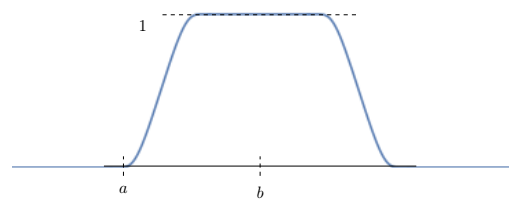
\includegraphics[scale=0.5]{img/caso1.png}} 

Entonces $\phi(a)=0$ y $\phi(b)=1$, de donde queda que $z(b)=0$. Tomando otra $\phi$ de esta forma
\centerline{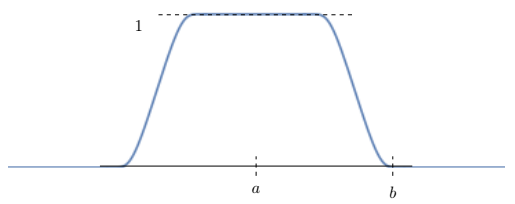
\includegraphics[scale=0.5]{img/caso2.png}} 

obtenemos que $z(a)=0$. Es decir, $y'(a)=y'(b)=0$.

\section{Sturm-Liouville: caso 2}

Para al siguiente caso tenemos que definir primero la \textit{delta de Dirac}.

\medskip

\begin{definition}
Dado $\alpha\in(a,b)$, definimos la función $\funcion{\delta_\alpha}{\sobolev{-1}}{\R}$
\[
\delta_\alpha(y)=y(\alpha), \espacio \delta_\alpha\in\sobolev{1}, \;\; \delta_\alpha\notin\sobolev{0}
\]
A $\delta_\alpha$ se le llama $\delta$ de Dirac.
\end{definition}
\begin{remark}
Nótese que esta función simplemente es otra forma de denotar la evaluación en $\alpha$, que usamos para indicar en qué punto ($\alpha$) de una cuerda ($y$) colgamos una masa $c$. 
\end{remark}

Ahora pasamos al siguiente caso, donde suponemos que $R(\phi)=c\delta_\alpha(\phi)=c\phi(\alpha) \espacio \forall \phi\in\sobolev{1}\subset\continuas$, con $a<\alpha<b$. Con esta nueva $R$, vemos otra vez la ecuación \ref{condicion1} con $z=y'$:
\[
\integral{a}{b}{z(x)\phi'(x)dx}+\integral{a}{b}{q(x)y(x)\phi(x)dx}=c\phi(\alpha)
\]
donde solo sabemos que $z\in\lebesgue{2}$ e $y\in\sobolev{1}$ y $z$ no tiene por qué tener derivada débil ya que la expresión anterior no coincide con la de la definición. 

Si ahora considero el intervalo $(a,\alpha)$ y tomo $\phi\in\mathcal{D}(a,\alpha)$, tenemos que $\phi(\alpha)=0$ y
\[
\integral{a}{b}{z(x)\phi'(x)dx}+\integral{a}{b}{q(x)y(x)dx}=0
\]
Luego $z\in\sobolev[a,\alpha]{1}$, que tiene un representante continuo $z_1\in\mathcal{C}[a,\alpha]$. De forma análoga, obtenemos $z_2\in\mathcal{C}[\alpha,b]$. Si definimos $z'$ como la unión de $z_1'$ y $z_2'$:
\[
z'(x)= \left\{
\begin{array}{cc}
z_1'(x) & x\in(a,\alpha) \\
z_2'(x) & x\in(\alpha,b)
\end{array}
\right.
\]
¿y qué pasa con $z'(\alpha)$? No pasa nada, porque $\{\alpha\}$ tiene medida nula asi que no hace falta definirla en ese punto. Además, $z'\in L^2(a,\alpha)$ y $z'\in L^2(\alpha,b)$, luego $z'\in\lebesgue{2}$ por la misma razón. 

Como $z'$ no es la derivada débil de $z$ en $(a,b)$, solo podemos decir que
\[
\integral{a}{b}{z'(x)\phi(x)dx}+\integral{a}{b}{z(x)\phi'(x)dx}=0 \espacio \forall \phi\in\mathcal{D}(a,\alpha) \text{ y } \forall \phi\in\mathcal{D}(\alpha,b)
\]
Y en ese caso, $z'(x)=-q(x)y(x) \;\; \casipordoquier$. 

Como vemos, este es el origen de la cuestión, tenemos una función $z'$, que sabemos que es una derivada, pero es una derivada \textit{extraña}, ya que es débil en $(a,\alpha)$ y $(\alpha,b)$, coincide en casi todo punto con $-q(x)y(x)$, pero no es una derivada débil en $(a,b)$. 

Por la condición de punto crítico, tenemos que:
\[
\integral{a}{b}{z_1(x)\phi'(x)dx}+\integral{a}{b}{q(x)y(x)\phi(x)dx}=0 \espacio \forall\phi\in\mathcal{H}^1(a,b)
\]
Si $phi(x)=0\quad\forall x\geq\alpha$,
\[
\integral{a}{\alpha}{z_1(x)\phi'(x)dx}+\integral{a}{\alpha}{q(x)y(x)\phi(x)dx}=0
\] 
Si igual que en el caso anterior, consideramos $\phi\in\mathcal{D}(\R)$ y aplicamos integración por partes al primer término:
\[
\integral{a}{\alpha}{z_1(x)\phi'(x)dx}=z_1(x)\phi(x)\Big|_a^\alpha-\integral{a}{\alpha}{q(x)y(x)\phi(x)dx}
\]
Cogiendo la $\phi$ de forma que $\phi(a)=1$ y $phi(x)=0\quad\forall x\geq\alpha$ y sustituyendo en la expresión anterior, obtenemos que:
\[
-z_1(a)\phi(a)=0 \Rightarrow z_1(a)=0
\]

Análogamente se prueba que $z_2(b)=0$.

% A partir de aquí no tiene sentido, supongo que está incompleto
Si ahora usamos eso en la expresión:
\[
\integral{a}{b}{z(x)\phi'(x)dx}+\integral{a}{b}{q(x)y(x)\phi(x)dx}=0
\]
Pero claro, el primer término lo podemos partir en dos integrales diferentes:
\[
\integral{a}{b}{z(x)\phi'(x)dx}=\integral{a}{\alpha}{z(x)\phi'(x)dx}+\integral{\alpha}{b}{z(x)\phi'(x)dx}
\]

\subsection{CLASE 31 MARZO}

